\chapter{АЛГОРИТМ МОДУЛЯ СКАНИРОВАНИЯ}\label{chap:algorithms}
    \section{Этапы работы алгоритма}
        Задача алгоритма заключается в преобразовании входных данных -- видео процесса сканирования и dxf файла с заданным контуром -- в gcode файл. Gcode файл это последовательность инструкций для принтера написанных особым образом. Файл формата dxf это векторное изображение некоторого произвольного рисунка, которое необходимо нанести на изделия в сцене.
        В целом алгоритм модуля состоит из четырёх операций:
        \begin{enumerate}
            \item Обработка видео/Получение облака точек
            \item Поиск объектов в облаке
            \item Подготовка dxf файла
            \item Генерация gcode файла
        \end{enumerate}
        
        Последовательность операций отражена в блок-схеме на рисунке \ref{pic:general_scheme}.
        \begin{figure}[H]
            \centering
            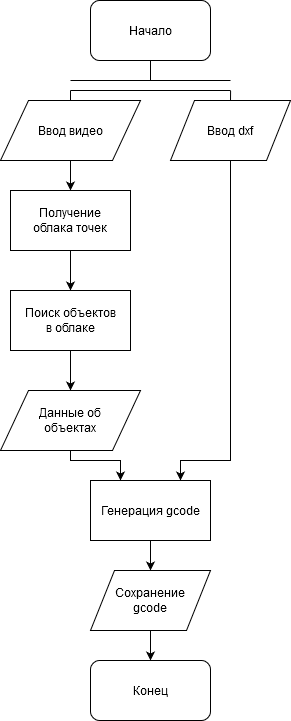
\includegraphics[width=0.4\linewidth]{general scheme}
            \caption{Обобщённая блок схема алгоритма модуля}
            \label{pic:general_scheme}
        \end{figure}
         При запуске алгоритма на вход передаются видео со сканера и dxf файл. После этого запускаются этапы обработки видео и dxf файла. Эти этапы независимы друг от друга и могут выполняться параллельно. Этап обработки видео включает в себя предобработку каждого кадра, затем выделение лазера в кадре, расчёт координат по формулам из главы \ref{chap:math}. Результатом этого этапа является облако точек сцены. Оно передаётся в следующий блок для поиска объектов. Цель этого этапа в получении положений и ориентаций объектов в сцене. Затем данные об объектах и подготовленный рисунок передаются в последний блок алгоритма, где из них генерируется файл инструкций для принтера которые задают последовательность печати рисунка из dxf файла на каждый найденный объект в сцене.
    \section{Блок обработки видео}
        Как уже было сказано, блок обработки видео включает в себя следующие шаги, которые выполняются для каждого кадра видео:
        \begin{enumerate}
            \item Предобработка кадра
            \item Выделение лазера
            \item Расчёт координат
        \end{enumerate}
        
        \begin{wrapfigure}{r}{0.5\linewidth}
            \centering
            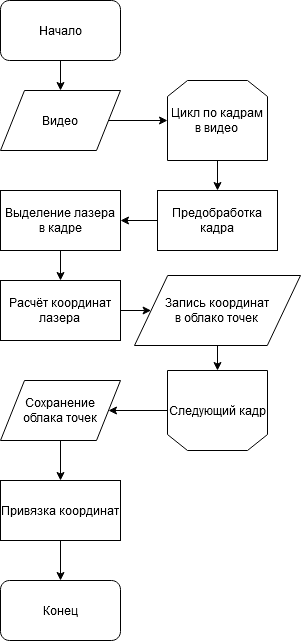
\includegraphics[height=0.45\textheight, keepaspectratio]{video_processing}
            \caption{Обобщённая блок схема обработки видео}
            \label{pic:video_processing}
        \end{wrapfigure}
        После этого облако точек сохраняется в памяти и производится привязка координат к системе принтера. Этот этап необходим, потому что в виду аппаратных ограничений сканирование в общем случае начинается в произвольном месте до рабочей поверхности и получить точную координату не представляется возможным.
        \sloppy Результатом работы алгоритма становится облако точек, представляющее из себя матрицу размерностью $ (\mbox{\textit{количество кадров}}\times\mbox{\textit{ширина кадра}}) $ где в каждой ячейке записана координата соответствующая этой точке. Таким образом облако точек одновременно является картой глубины сцены.
        
        \subsection{Предобработка}
            \begin{wrapfigure}{l}{0.42\linewidth}
                \centering
                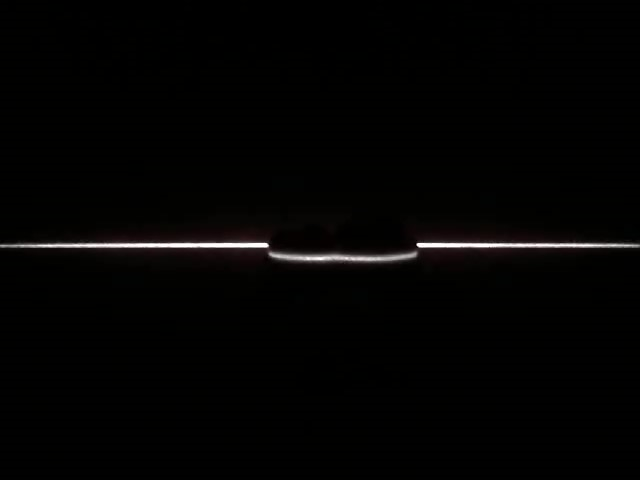
\includegraphics[width=0.4\textwidth]{frame_sample}
                \caption{Пример кадра из видео}
                \label{pic:frame_sample}
            \end{wrapfigure} 
            Перед тем как выделить на изображении лазер, необходимо провести предобработку, которая сгладит шумы в кадре и уберёт большинство лишней информации. Первым шагом необходимо обрезать видео по заранее установленной области интереса. Вне этой области заранее гарантировано отсутствие полезной информации, т.е. вне этой области нет рабочей зоны. 
            
            Затем к изображению применяется фильтр гаусса \cbox{пояснение что это?}, что размывает картинку. Это делается с целью <<размешать>> \cbox{пояснить} шум имеющийся на изображений и сгладить резкие переходы, что поможет на следующем шаге. 
            
            После этого с полученного изображения снимается <<маска>> -- то есть изображение бинаризируется. В таком изображении единицами обозначена область, которую мы хотим оставить, а нулями область, которую мы хотим отбросить. Для получения маски предусмотрено два подхода на выбор -- бинаризация по заданному пороговому значению и бинаризация с порогом по Оцу. Последняя хороша тем, что позволяет избежать необходимость ручного подбора порогового значения. 
            
            Метод Оцу применим к изображениям на гистограмме которых есть только два пика. Хорошее пороговое значение для таких изображений находится между этими двумя пиками\cite{opencvTHRESH}.
            
            Это идеально подходит для нашего случая. Такая маска единицами пометит области на изображении, в которых с наибольшей вероятностью находится лазер, а нулями области, где лазера почти наверняка нет.
            
            Последним шагом является применение маски к обрезанному изображению, что представляет собой простое поэлементное умножение. Таким образом мы получаем изображение, в котором область, где почти наверняка лазера нет, состоит из пикселей значение которых равно нулю, остальная же часть остаётся нетронутой.

            Это изображение затем передаётся в следующий блок алгоритма для выделения лазера.

        \subsection{Выделение лазера}
            Для постановки задачи выделения лазера в первую очередь необходимо определить, что из себя представляет линия лазера на изображении. В нашем случае линия лазера в кадре располагается параллельно оси $ X $ изображения. Интенсивность в профиле лазера, т.е. сечении в перпендикулярном линии направлении, соответствует Гауссовому распределению\cite{Qi2013, Molder2014} с некоторым шумом. Пик интенсивности, без учета шума, соответствует центру полосы лазера.
            \begin{wrapfigure}{l}{0.4\linewidth}
                \centering
                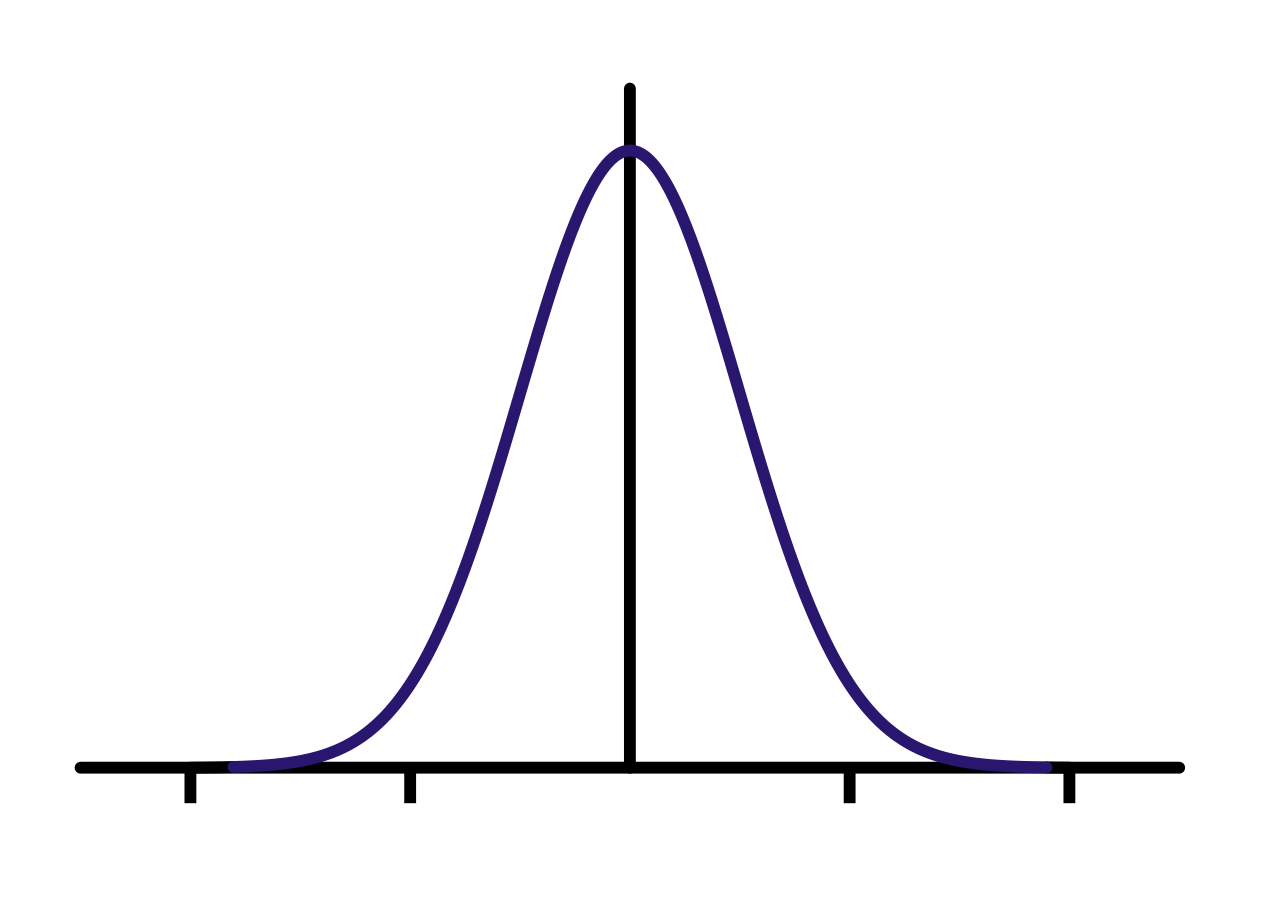
\includegraphics[width=0.38\textwidth]{gauss_profile}
                \caption{Распределение Гаусса}
                \label{pic:gauss_profile}
            \end{wrapfigure}
            Таким образом задача выделения лазера на изображении в первом приближении сводится к определению пика интенсивности для каждого профиля лазера, то есть в нашем случае для каждой колонки пикселей изображения.
            
            Однако задача усложняется наличием шумов на изображении, которые постоянно искажают профиль интенсивности лазера. Причинами шумов могут являться светочувствительный сенсор в камере, явление самозасвета лазера, неподходящие условия окружения, программная обработка изображения на этапе кодирования-декодирования и так далее.
            
            Помимо этого в общем случае линия лазера на изображении не является непрерывной. Разрывы могут возникать в следствии недостаточной контрастности лазера или попадания линии лазера в слепую зону. Эта проблема также требует какого-то решения.
            
            Рассмотрим существующие алгоритмы для выделения лазера на изображении и как они справляются с упомянутыми проблемами.
            
            Критерии сравнения/решаемые задачи
            \begin{itemize}
                \item шум
                \item разрывы
                \item изменение яркости
                \item скорость выполнения
                \item точность определения
            \end{itemize}
            
            \paragraph{Метод максимальной интенсивности}
                Данный метод находит максимум интенсивности в каждой колонке изображения и считает этот максимум центром лазера. Этот метод обладает пиксельной точностью.
            
            \paragraph{Laplacian of Gaussian}
                На реальных изображениях пик профиля лазера как правило срезан, поэтому метод максимумов в данном случае не даёт максимальной точности\cite{Molder2014}. 
                 
                \begin{wrapfigure}{r}{0.4\linewidth}
                    \centering
                    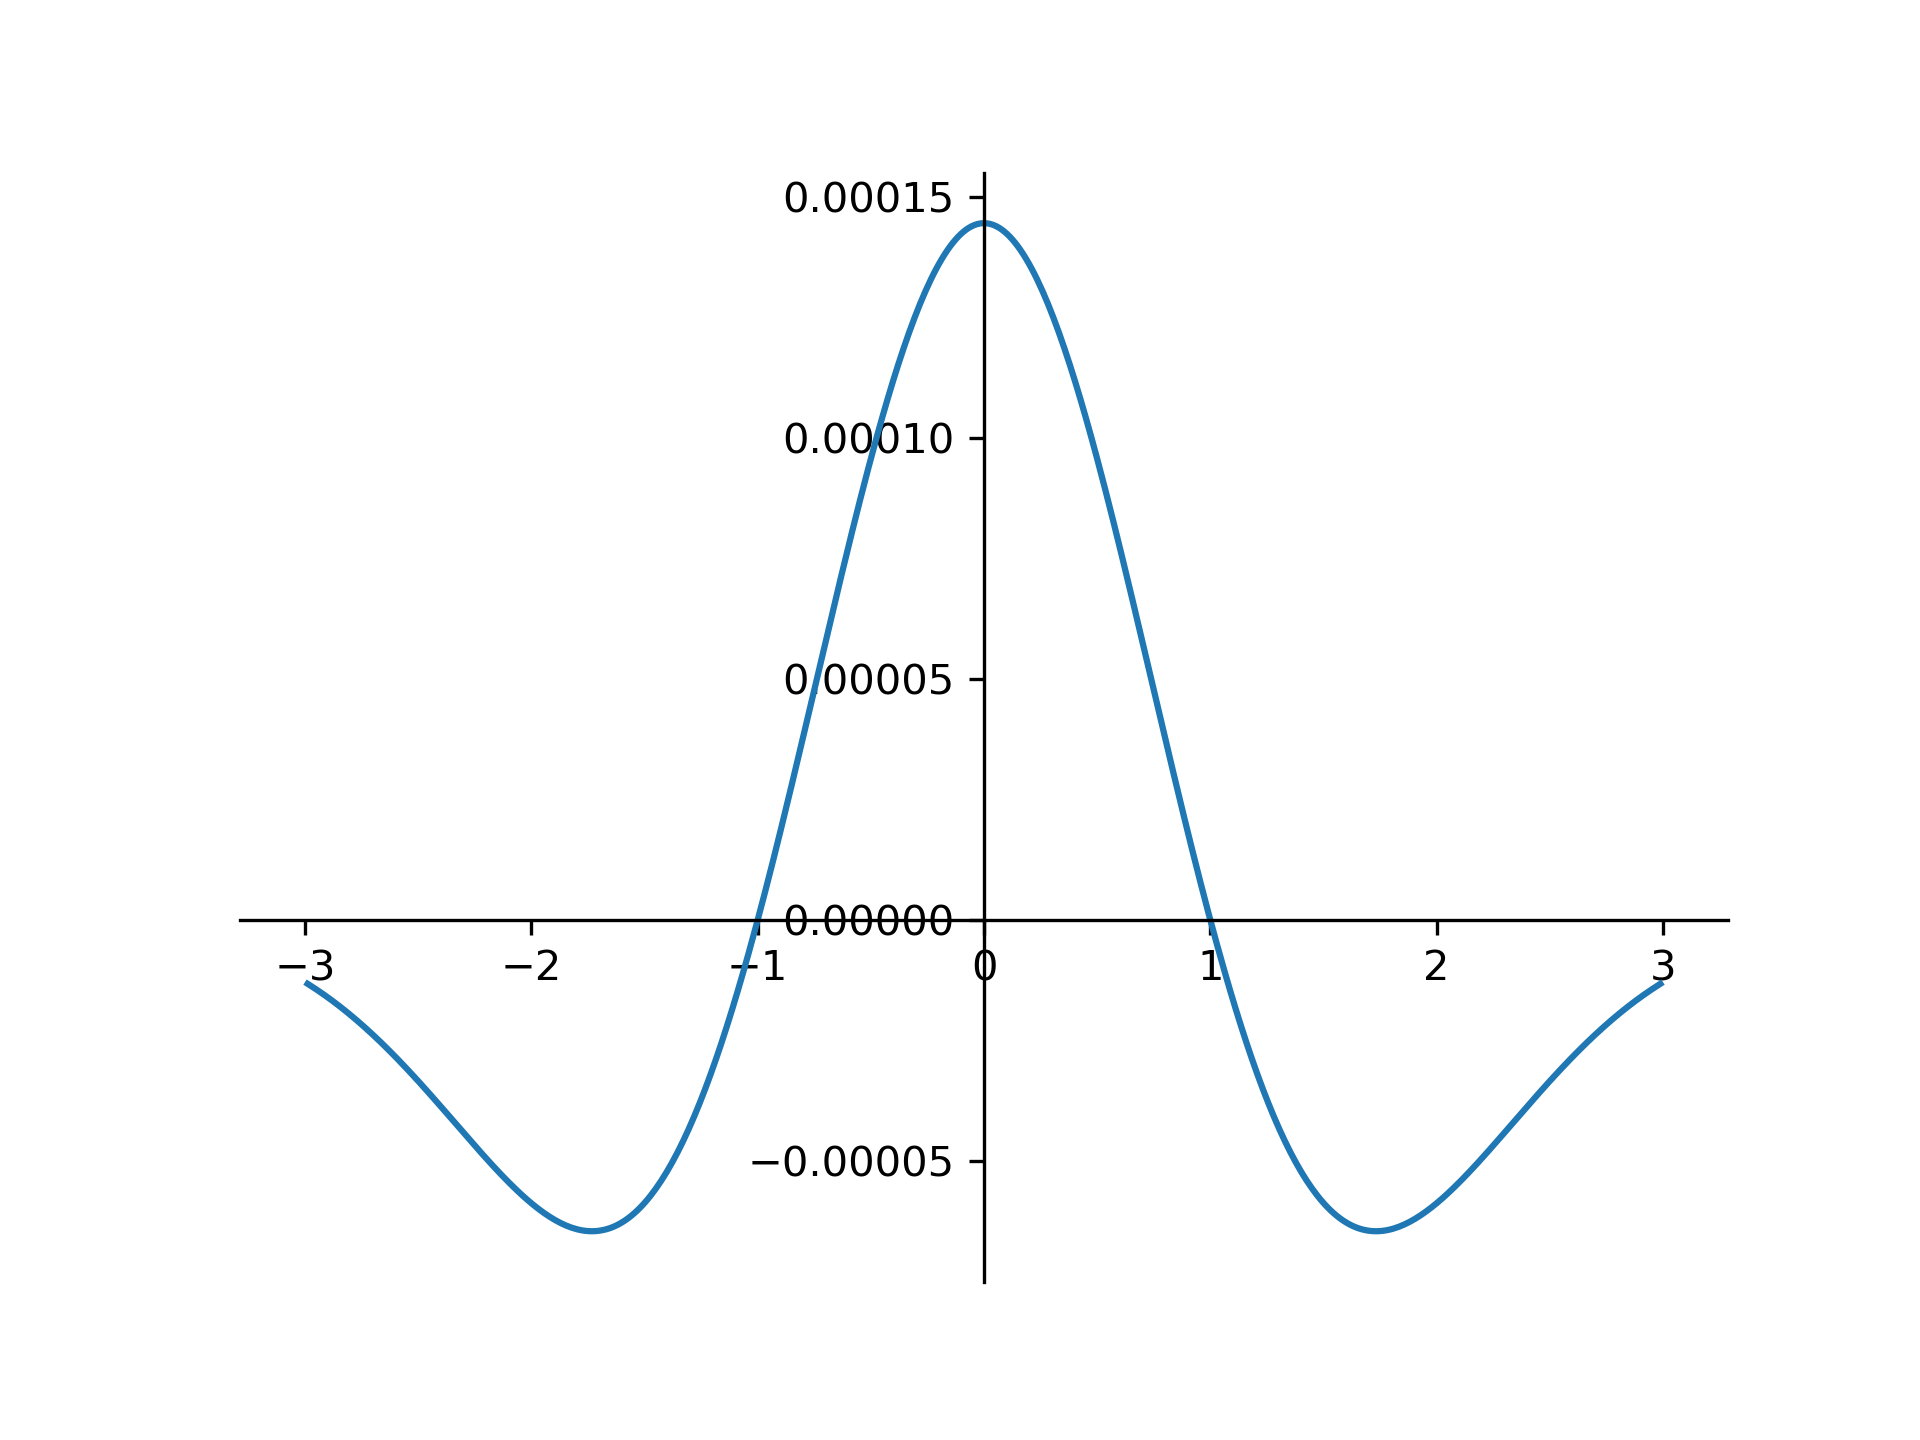
\includegraphics[width=0.38\textwidth]{gauss_second_order}
                    \caption{Профиль интенсивности лазера после LoG преобразования}
                \end{wrapfigure}
                Чтобы это преодолеть к изображению можно применить LoG преобразование, то есть применить гауссовое размытие, после чего вычислить вторую производную по изображению. Полученный результат инвертировать. Данный метод в общем случае используется для выделения краёв и линий на изображении\cite{Steger2000}. Для использования этого метода необходимо выбрать дисперсию $ \sigma $ гауссового распределения. При малых $ \sigma $ таким образом возможной найти линии малой толщины, при б\'{о}льших $ \sigma $ наоборот, но одновременно за одно преобразование находить линии сильно отличающейся толщины невозможно.
                Параметр $ \sigma $ можно найти эмпирически, но можно воспользоваться оценкой $ \sigma > \dfrac{w}{\sqrt{3}} $ из работы \cite{Steger2000}, где $ w $ -- ширина линии лазера в пикселях.
                
                Данный метод также обладает пиксельной точностью
                
                Недостатками этого метода являются ухудшение детектирования на краях, так как происходит размытие изображения, необходимо больше времени на обработку по сравнению с методом максимумов и ggm, невозможность одновременно определять линии разной толщины (такая ситуация возникает, когда измеряются высокие объекты и линия лазера в кадра становится заметно шире).

            
            \paragraph{Квадратичная аппроксимация}
                Предыдущие два метода возможно улучшить и привести точность к субпиксельной\cite{Molder2014}. Если рассмотреть профиль интенсивности лазера по пикселям, то в общем случае действительный максимум приходится на значение между пикселей. Также можно заметить что в окрестности максимума профиль представляет собой некоторую параболу $ y = ax^2 + bx + c $. Взяв три точки -- точку перед максимумом, точку максимума, точку после максимума -- легко найти коэффициенты этой параболы и, соответственно, вершину, которая будет являться действительным максимумом.
                
                Данный метод лучше применим к LoG трансформации, т.к. уже было сказано, что изначальный профиль лазера как правило обрезан при вершине. Однако в определённых условиях можно применять данный подход и для метода максимумов.
            
            \paragraph{Gray-Gravity Method} \cbox{и как это по русски?}
                Метод субпиксельной точности\cite{Li2017}. 
                По данному методу центр лазера $ (i_c, j_c) $ рассчитывается как <<центр масс>> интенсивностей в колонке $ j_c $ изображения по формуле
                \begin{equation}
                    i_c = \left(\sum\limits_{i=1}^{H}I(i, j_c)\cdot i\right)\cdot\left(\sum\limits_{i=1}^{H}I(i, j_c)\right)^{-1}
                \end{equation}
                где $ H $ -- высота кадра в пикселях, $ I(i, j_c) $ интенсивность $ i-\textit{го} $ пикселя в колонке.
                
                Этот метод крайне чувствителен к шумам, поэтому несмотря на субпиксельную точность его применение в задачах требующих высокой точности нежелательно.
                
                Однако данный метод очень быстр, поскольку вычисления простые.
                
            \paragraph{Improved Gray-Gravity Method}
                Улучшенный вариант предыдущего метода\cite{Li2017}. Предполагает два основных шага -- предварительное определение центра лазера методом центра масс, затем уточнение координаты.
                
                Уточнение координаты происходит следующим образом:
                С помощью методом скользящих наименьших квадратов находится касательная, нормаль и кривизна линии в точке предварительного центра. На основе этих значений подбирается прямоугольная область ограничивающая множество точек для расчётов. Затем рассчитывается отклонение действительного центра лазера от предварительного на основе интенсивности точек в регионе и их расстояния до линии пересекающей предварительный центр по направлению касательной в этой точке.
                
                Достоинством этого метода является то, что он учитывает направление линии лазера в кадре и кривизну линии. Предыдущие методы предполагают что лазер параллелен оси $ x $ изображения, из-за чего теряют несколько в точности.
                
                Однако данный метод сложнее реализовать и он также требует больше вычислений чем предыдущие методы.
                
            \paragraph{Другие методы}
                Кроме упомянутых методов существуют множество других. В частности Gaussian Fitting\cite{Qi2013} и Usamentiaga Method\cite{Usamentiaga2012}.
                
                Gaussian Fitting основан на статистическом анализе метода Штегера, описанном в работе \cite{Steger2000}. В работе \cite{Qi2013} выдвигается математический аппарат для определения параметров распределения лазера на основе данных с изображения, в частности соотношения сигнал/шум.
                
                Суть данного метода заключается в том, чтобы отыскать реальное распределение интенсивности лазера на изображении без влияния шума и таким образом найти реальный центр лазера.
                
                Достоинствами этого метода являются высокая устойчивость к шумам и высокая точность определения центра лазера.
                
                Недостатком является большое время выполнения даже для одного изображения, что не позволяет использовать этот метод в задачах требующих быстрого выполнения.
                
                Usamentiaga method 
            
            \paragraph{Выбранный метод}
            
        \subsection{Привязка координат}
            Ранее было сказано, что в виду аппаратных ограничений видео сканирования в общем случае начинается в неопределённый момент перед рабочей зоной. При этом нет возможности узнать координату сканера в момент начала записи видео. Это порождает проблему несоответствия рассчитанных в процессе обработки координат и реальных. Таким образом необходимо разработать алгоритм, который позволял бы по данным с видео определить необходимое смещение координат.
            
            Основная идея такого алгоритма состоит в том, что необходима уникальная метка-идентификатор, имеющая заранее известную координату. Такая метка и алгоритм должны удовлетворять следующим требованиям:
            \begin{itemize}
                \item Лёгкое определение по входному видео
                \item Устойчивость к ложноположительным срабатываниям
                \item Лёгкое внедрение в конструкцию
                \item Минимальное влияние на общее время работы алгоритма
            \end{itemize}

            Предлагается использовать рельефные идентификаторы на столе, которые будут образовывать некоторый паттерн схожий с идеей штрихкода. Таким образом после сканирования в облаке точек сцены будет видна данная метка, которую возможно распознать программными методами и рассчитать необходимое смещение.
            
            В конечном итоге идентификатор представляет собой ряд меток расположенных на некотором заданном расстоянии друг от друга. Метки же в свою очередь представляют некоторую прямоугольную поверхность заданной ширины на определённой высоте от стола. Высота от стола для всех меток одинаковы, остальные параметры произвольны.
            
            Алгоритм перебирает профили сцены в облаке точек и сравнивает их на соответствие заданному идентификатору. Как только алгоритм находит подходящий профиль рассчитывается необходимое смещение, которое применяется ко всем координатам в облаке.
            
    \section{Блок поиска объектов}
        Задача поиска объектов в произвольном облаке точек одна из сложнейших. Такие задачи в настоящее время пытаются решить с использованием нейронных сетей и <<искусственного интеллекта>>. На данный момент нет стандартных подходов к решению этой задачи.
        
        Однако в нашем случае задача значительно упрощается по следующим причинам:
        \begin{itemize}
            \item у нас есть карта глубины с прямым соответствием пикселей и реальных координат
            \item объекты довольно простые (\cbox{типа плоские})
            \item необходимо распознать только верхнюю часть объектов
        \end{itemize}
        Поэтому мы можем перевести задачу из распознавания объектов в пространстве в распознавание замкнутых контуров на изображении.
        
        \cbox{БЛОК-СХЕМА}
        
        На вход алгоритму подаётся карта глубины сцены, на которой видны изделия. Применив к изображению алгоритм watershed мы найдём контур для каждого объекта, даже в случае их прямого соприкосновения. Поскольку карта глубины даёт прямое соответствие между пикселями и координатами, то наш контур задаётся некоторым пространственным многоугольником. Отбросив $ z $ координату, получим проекцию контура на плоскость. Затем можно расчитать моменты этого контура и получить его центроиду. Так же через моменты можно найти ориентацию контура в пространстве (поворот вокруг центра), это эквивалентно вписыванию эллипса в контур и нахождения угла наклона главной диагонали.
        
        Таким образом для каждого найденного контура программой формируется объект содержащий следующие данные:
        \begin{itemize}
            \item область в облаке точек, содержащую только этот контур
            \item координату центра объекта в плоскости
            \item ориентацию объекта в плоскости
        \end{itemize}
        Область в облаке сохраняется с целью оптимизации по времени алгоритма проекции рисунка на рельеф.
        
        \begin{figure}[H]
            \begin{subfigure}{0.5\linewidth}
                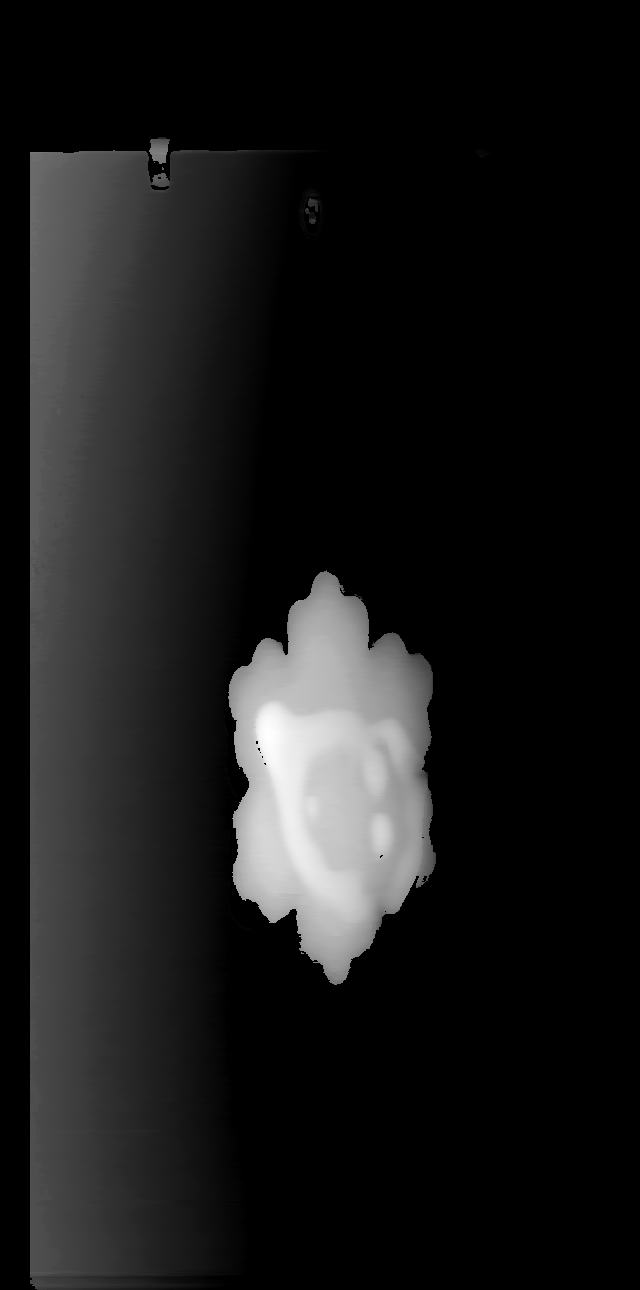
\includegraphics[width=\linewidth]{depthmap}
                \caption{Карта глубины поданная на вход}
            \end{subfigure}
            \begin{subfigure}{0.5\linewidth}
                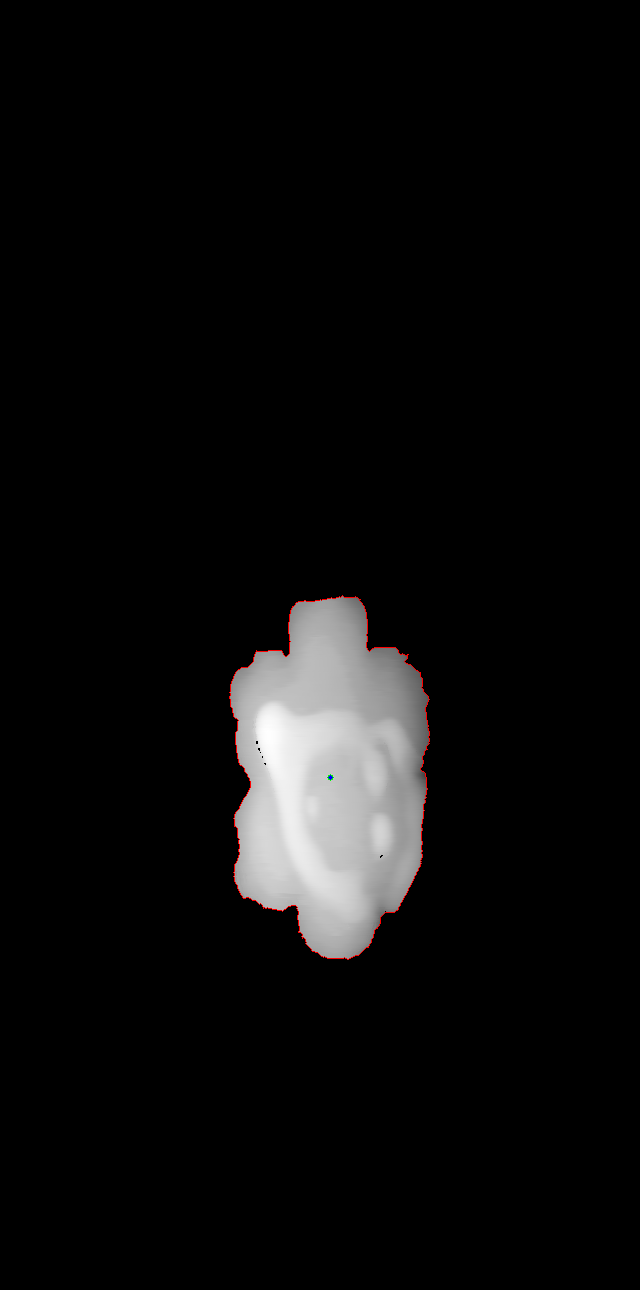
\includegraphics[width=\linewidth]{found_objects}
                \caption{Обнаруженные объекты}
            \end{subfigure}
            \caption{Пример работы алгоритма}
        \end{figure}
        
    \section{Блок генерации gcode}
        3D-принтеры, и прототип в частности, не способны описывать сложные кривые в пространстве. Возможно описывание окружностей и, в некоторых случаях, простейших сплайнов только в горизонтальной плоскости. Это существенное препятствие в нашем проекте, так как сопло печатающего элемента должно огибать сложную поверхность. Также dxf рисунок может задавать контуры сложной формы даже в плоскости. Для преодоления данных ограничений было решено реализовать слайсер-алгоритм решающий эту задачу.
        
        \begin{figure}[H]
            \centering
            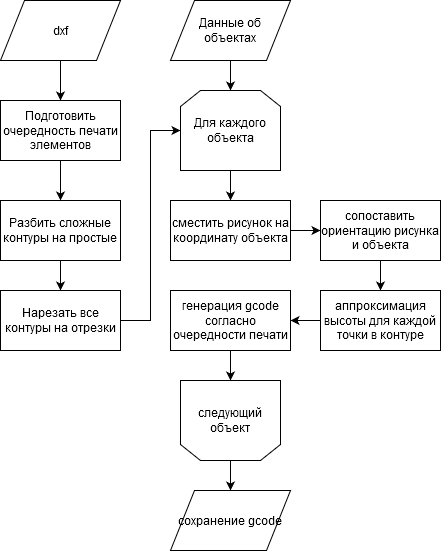
\includegraphics[width=0.5\linewidth]{gcoder}
            \caption{Блок-схема генератора gcode}
            \label{pic:gcoder}
        \end{figure}
        
         На вход алгоритма поступают данные об объектах и рисунок. В первую очередь происходит обработка dxf файла -- формируется очерёдность нанесения элементов рисунка в зависимости от их примыкания и расположения в структуре файла; сложные элементы (например, сплайны) разбиваются на более простые; все элементы <<нарезаются>> на отрезки определённой длины, заданной пользователем.
         
         Затем обработанный файл комбинируется с данными о каждом объекте. Для каждой точки в контуре аппроксимируется соответствующая высота на основе данных облака. В процессе разработки были опробованы три варианта аппроксимации -- выбор ближайшей точки, среднее \textit{k}-ближайших соседей и метод скользящих средних квадратов.
         
         \paragraph{Ближайшая точка}
         По данному методу для заданной $ (x_p,y_p) $ координаты в облаке ищется аппроксимирующая точка $ (x_a, y_a, z_a) $ для которой $ (x_a-x_p)^2 + (y_a-y_p)^2 $ есть минимум среди всех точек в облаке. (т.е. ищется точка, евклидово расстояние до которой в проекции на плоскость минимально) \cbox{выбрать формулировку}
         
         \paragraph{\textit{k}-ближайших соседей}
         По данному методу выбирается \textit{k} точек, расстояние до проекции которых от необходимой точки минимально. Затем вычисляется среднее координаты $ z $ этих точек. Полученное значение является аппроксимированной высотой искомой точки.
         
         \paragraph{Скользящие наименьшие квадраты}
         Это метод поиска некоторой полиномиальной функции, которая аппроксимирует данные с наименьшей квадратичной ошибкой в окрестности заданной точки \cite{Veerabhadra2017}. То есть имея множество $ n $ точек $ \{M_i(x_i, y_i, z_i)\}_{i=1}^{n} $ и опорную точку $ M_p(x_p, y_p) $ необходимо найти коэффициенты $ c_{kl} $ следующей функции
         \begin{equation}
             f(x,y)=\sum\limits_{k=0}^{p}\sum\limits_{l=0}^{q}c_{kl}x^ky^l,
         \end{equation}
         где $ p $, $ q $ -- максимальная степень $ x $ и $ y $ переменных соответственно.
         Для нахождения коэффициентов необходимо решить задачу минимизации следующей функции
         \begin{equation}
             E = \sum\limits_{i}^{n}w_i(r_i)\left(\sum\limits_{k=0}^{p}\sum\limits_{l=0}^{q}c_{kl}x_i^k y_i^l - z_i\right),
         \end{equation}
         где $ w_i $ -- весовой коэффициент задающийся следующим образом
         \begin{equation}
            w_i(r_i) = 
                     \begin{cases}
                         1-6r_i^2+8r_i^3-3r_i^4, &r_i \le 1\\
                         0, &r_i > 1
                     \end{cases}
         \end{equation}
         где $ r_i $ -- нормализованное расстояние между опорной точкой $ M_p $ и точками $ M_i $ из множества, рассчитываемое по формуле
         \begin{equation}
             r_i = \sqrt{(x_i-x_p)^2 + (y_i-y_p)^2}\cdot R^{-1},
         \end{equation}
         где $ R $ -- радиус влияния, точки не входящие в этот радиус не имеют эффекта на аппроксимацию.
         Уравнения весовых коэффициентов выведены в работе \cite{LI2008}
         Минимизируя $ E $ и переписывая в матричном виде получаем следующее уравнение для коэффициентов функции $ f(x,y) $
         \begin{equation}
             c = \left[B^T W(M_p) B\right]^{-1} B^T W(M_p) z,
         \end{equation}
         где $ z = [z_1 ... z_n]^T$ -- вектор значений координат точек множества, $ B $ -- обобщённая матрица Вандермонда данных из $ (x,y) $ координат точек множества, в данном случае
         \begin{equation}
             B = 
             \begin{bmatrix}
                 1 & y_1 & x_1 & \cdots & x_1^p y_1^q\\
                 1 & y_2 & x_2 & \cdots & x_2^p y_2^q\\
                 \vdots & \vdots & \vdots & \ddots & \vdots\\
                 1 & y_n & x_n & \cdots & x_n^p y_n^q
             \end{bmatrix}
         \end{equation}
         
         Найдя таким образом аппроксимацию поверхности легко вычислить координату $ z $ искомой точки.
        
        \cbox{вставить картинки для разных методов}
        
        Из трёх рассмотренных методов последний поз
        
        
        
        
        
        
        
        